%************************************************
\chapter{Current mobile Platforms}\label{ch:m_plats} % $\mathbb{ZNR}$
%************************************************
Over the past few years competition between the different platform manufacturers has increased, leading to better products and features. In this chapter we will take a look at the most important players in mobile OS race, in alphabetical order.

\begin{figure}[H]
    \begin{center}
        {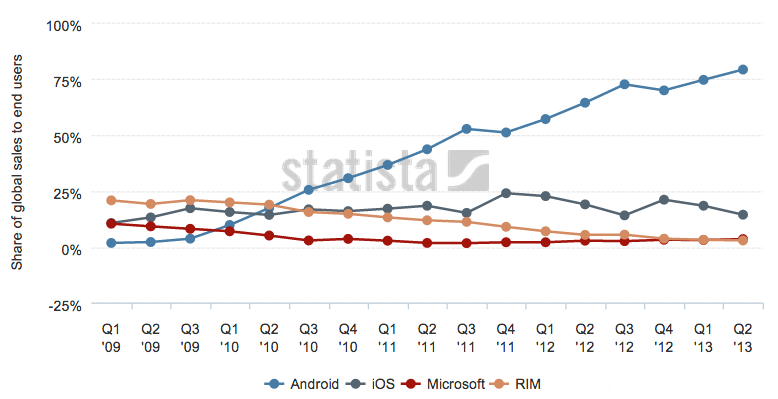
\includegraphics[width=1\linewidth]{gfx/statista-mobile}}
        \caption[Mobile OS share of global sales to end users]{Mobile OS share of global sales to end users\footnotemark}\label{fig:trend}
    \end{center}
\end{figure}
\footnotetext{Source: \url{http://www.statista.com/statistics/266136/global-market-share-held-by-smartphone-operating-systems}}\\

%***********************Ready
\section{Android}
\spacedlowsmallcaps{Android} is a Linux based operating system specially designed for touchscreen devices like smartphones or tablets. It began as the brain-child of a new company called Android, Inc. back in 2003. Since its inception, it has gained major popularity thanks to the plethora of devices that run it, giving users the option between low-budget and luxury phones and tablets. Its market share currently sits at over 75\% in terms of sales to end users.

\begin{quotation}
Android, Inc. was founded in Palo Alto, California in October 2003 by Andy Rubin (co-founder of Danger), Rich Miner (co-founder of Wildfire Communications, Inc.), Nick Sears (once VP at T-Mobile), and Chris White (headed design and interface development at WebTV) to develop, in Rubin's words "smarter mobile devices that are more aware of its owner's location and preferences". The early intentions of the company were to develop an advanced operating system for digital cameras, when it was realised that the market for the devices was not large enough, and diverted their efforts to producing a smartphone operating system to rival those of Symbian and Windows Mobile (Apple's iPhone had not been released at the time). Despite the past accomplishments of the founders and early employees, Android Inc. operated secretly, revealing only that it was working on software for mobile phones. That same year, Rubin ran out of money. Steve Perlman, a close friend of Rubin, brought him \$10,000 in cash in an envelope and refused a stake in the company.
\cite{wikipedia:android}
\end{quotation}

Google bought Android, Inc. in 2005 and made it a wholly owned subsidiary. The most important employees stayed and started working on what later would become the Android Operating System.

Up until the release of the first Android Device on October \nth{22}, 2008, Google conducted secret meetings with many handset and chip manufacturers to discuss the creation of a new consortium, the Open Handset Alliance, with the goal to develop open standards for mobile devices. The Alliance was unveiled on November \nth{5}, 2007.\footnote{\url{http://www.openhandsetalliance.com/press_110507.html}}


After the first device with Android, the HTC Dream, was released there has been a major surge of devices using Android. Hardware manufacturers from all over the world have chosen Android as their favourite operating system, not only for smartphones and tablets but also for embedded devices like the Cotton Candy Stick\footnote{\url{http://www.fxitech.com/technology/for-android/}} from FXI Technologies and even for gaming consoles like the Ouya\footnote{\url{https://www.ouya.tv/discover/}}. %They have gone the Android route to give their devices a robust and secure operating system.


The development of system features and other components has been done at a steady pace, releasing new versions of the OS every couple of months. The team has chosen to give colourful names to each release, always in alphabetical order and always named after a dessert or a sweet treat. A closer look at \autoref{fig:android1} and \autoref{fig:android2} should give you a better overview over the different versions of Android and what each of them brought forth.   

\begin{figure}
    \hbox{
        \hspace{-4em}
        {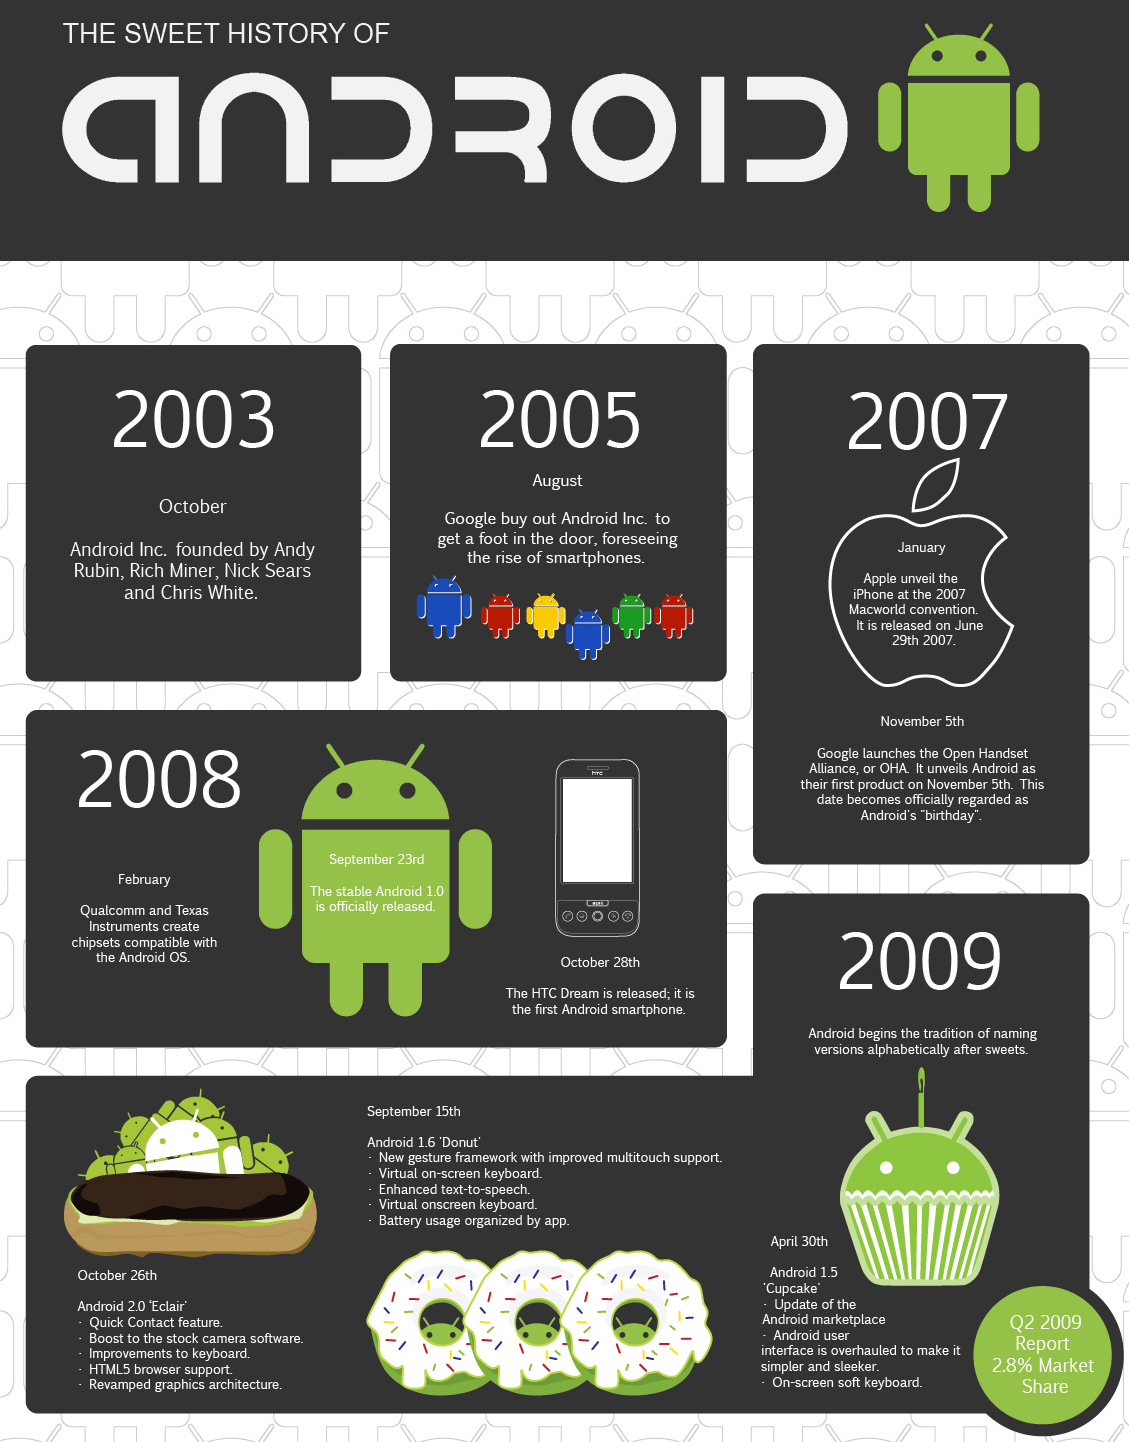
\includegraphics[width=1.5\linewidth]{gfx/android-history1}}
        \caption[Visual History of Android, Part 1]{Visual History of Android}\label{fig:android1}
    }
\end{figure}
\begin{figure}
    \hbox{
        \hspace{-12em}
        {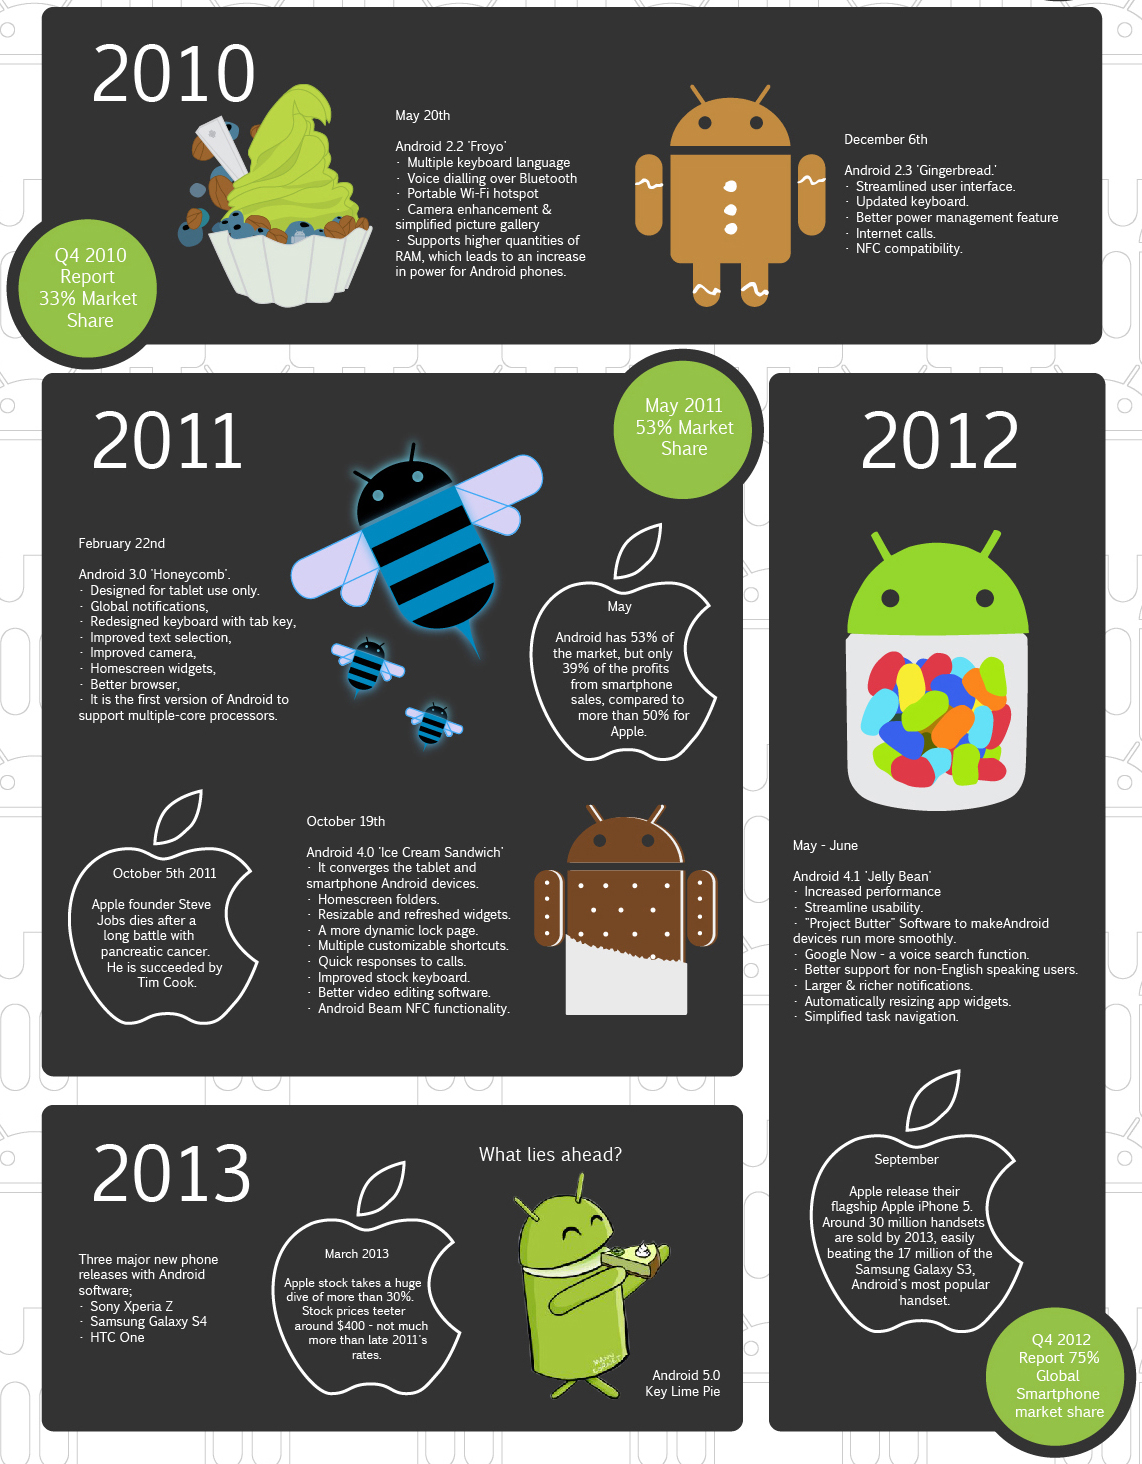
\includegraphics[width=1.55\linewidth]{gfx/android-history2}}
        \caption[Visual History of Android, Part 2]{Visual History of Android\footnotemark}\label{fig:android2}
    }
\end{figure}
\footnotetext{Source: \url{http://visual.ly/sweet-history-android}}\\

\subsection{The Android Open Source Project}
One of the best features and assets of Android is that it is 100\% Open Source. This allows everyone with the necessary knowledge to contribute to the development of the platform and also to modify it in every way you want.


This is exactly what the guys behind CyanogenMod\footnote{\url{http://www.cyanogenmod.org/}} have done. They took the regular Android Operating System and added many features and improvements to the core experience, making it the most popular unofficial Android OS.


But these types of modifications are not only common inside hobbyist communities, big corporations also contribute code to the Android Project. Some even modify the code so much, that it becomes almost unrecognisable. That is exactly what Amazon did. They took the Android OS and heavily modified it in order to install it in their Kindle Fire family of tablets.


Using an Open Source Model also guarantees Android an independent future from Google. Even if Google stops supporting \marginpar{Note: Google is unlikely to stop supporting Android} Android, the community will pick up the pieces and continue with its development and will guarantee its longevity.

%************************** 
\section{BlackBerry}
The Blackberry OS is proprietary mobile operating system developed by BlackBerry Ltd\marginpar{BalckBerry Ltd was until recently known as RIM (Research In Motion)} exclusively for its line of BlackBerry devices.

\begin{quotation}
Mike Lazaridis and Doug Fregin officially founded Research in Motion on March 7th, 1984 with a desire to commercialize Budgie, a system that wirelessly displayed information on a TV screen. It generated enough business to let RIM take on side projects, including a film barcode reader, but the real kick start was the arrival of one of the earliest wireless data networks, Mobitex. Software deals to support it led to the 1993 launch of RIMGate, the precursor to BlackBerry Enterprise Server, and wireless point-of-sale terminals in 1994.\\

For its first two decades, RIM often showed the traits of a scrappy startup. It had nothing to lose and was willing to turn its business model on a dime to stay afloat. More importantly, it also had a simple, overriding determination to spread wireless data to the masses, no matter how that would come to pass. That gave it a leg up over contemporary technology stalwarts like Apple, Microsoft and Palm, all of whom were at least slightly behind RIM in seeing the value of truly instant mobile communication.
\cite{fingas:2013}
\end{quotation}

RIM started the BlackBarry brand in March 2002 with the BackBerry 5800. Since then may improvements have been made to the operating system and the devices running it.
\begin{quotation}
The BlackBerry platform is perhaps best known for its native support for corporate email, through MIDP 1.0 and, more recently, a subset of MIDP 2.0, which allows complete wireless activation and synchronisation with Microsoft Exchange, Lotus Domino, or Novell GroupWise email, calendar, tasks, notes, and contacts, when used with BlackBerry Enterprise Server.
\cite{wikipedia:bb}
\end{quotation}

\begin{quotation}
In 2005, the 8700 series took the 7100's sleeker aesthetic to the high-end; for many, it was the first modern BlackBerry, where a polished design, phone features and a full keyboard were all in one device. Not that RIM could rest on its laurels. Nokia, Palm and others had thrown themselves wholeheartedly into smartphones, and Microsoft's launches of Pocket PC 2002 and Windows Mobile provided a start for smartphone makers that would eventually play important roles, like HTC.
\cite{fingas:2013}
\end{quotation}


BlackBerry was once the King of Smartphones, surpassing its competitors by quite some margin, specially in the enterprise sector; but now BlackBerry is fighting for its life, having lost over \$1 Billion last quarter, mainly due to their failure to sell their latest flagship device, the BlackBerry Z10, in the expected quantities.\footnote{\url{http://arstechnica.com/business/2013/09/true-to-its-recent-prediction-blackberry-lost-over-1-billion-last-quarter/}} It now hopes to recover by selling the company.\footnote{\url{http://arstechnica.com/business/2013/08/blackberry-announces-that-it-may-sell-the-company/}}


The BlackBerry OS hasn't been very popular among developers, either. With the launch of iOS and Android and their easy to use SDKs most developers flocked to the other platforms, leaving BlackBerry a barren territory, so much so that a single company developed 47,000 of the 120,000 applications currently available for BlackBerry devices.\footnote{\url{http://arstechnica.com/gadgets/2013/08/one-developer-makes-over-47000-of-blackberry-10s-120000-apps/}} As expected, market share has steadily fallen, to the point where it now sits at just under 3\% of total sales to end users.
  

%**************
\section{iOS}
\spacedlowsmallcaps{iOS} is a Unix-based (BSD) mobile operating system designed by Apple exclusively for its mobile devices, the iPhone\textregistered{} and the iPad\textregistered. When first unveiled adoption rates for iOS powered devices skyrocketed, leaving it with a healthy 17\% share of global sales to end users by the end 2009, almost as much as BlackBerry. Since then, demand for new iOS devices has maintained between 13\% and 24\%, always growing a little whenever a new iPhone is announced.

\begin{quotation}
    The operating system was unveiled with the iPhone at the Macworld Conference \& Expo, January 9, 2007, and released in June of that year. At first, Apple marketing literature did not specify a separate name for the operating system, stating simply that the "iPhone runs OS X". Initially, third-party applications were not supported. Steve Jobs' reasoning was that developers could build web applications that "would behave like native apps on the iPhone". On October 17, 2007, Apple announced that a native Software Development Kit (SDK) was under development and that they planned to put it "in developers' hands in February". On March 6, 2008, Apple released the first beta, along with a new name for the operating system: "iPhone OS".
Apple had released the iPod Touch, which had most of the non-phone capabilities of the iPhone. Apple also sold more than one million iPhones during the 2007 holiday season. On January 27, 2010, Apple announced the iPad, featuring a larger screen than the iPhone and iPod Touch, and designed for web browsing, media consumption, and reading iBooks.
In June 2010, Apple rebranded iPhone OS as "iOS". The trademark "IOS" had been used by Cisco for over a decade for its operating system, IOS, used on its routers. To avoid any potential lawsuit, Apple licensed the "IOS" trademark from Cisco.
\cite{wikipedia:ios}
\end{quotation}

The history of iOS has been very straight forward and a new version has been unveiled every year. Unlike Google, Apple doesn't use code-names for every version of iOS, they just carry their version number. You can take a look at \autoref{fig:ios} for a more detailed description of every iOS version released until now.  

\begin{figure}[H]
    \begin{center}
        {\includegraphics[width=.95\linewidth]{gfx/ios-history}}
        \caption[Visual History of iOS]{Visual History of iOS\footnotemark}\label{fig:ios}
    \end{center}
\end{figure}
\footnotetext{Source: \url{http://visual.ly/history-ios}}\\

\subsection{Jailbreaking}
The very strict guidelines and restrictions imposed by Apple on their mobile operating system have led to many developers and hackers to come up with ways to circumvent them and use their rightfully owned devices to their full potential. This method is called \emph{Jailbreaking}\footnote{\url{http://en.wikipedia.org/wiki/IOS_jailbreaking}} \marginpar{Jailbreak: In other words, release their devices from the fictional jail imposed by Apple.} and it give users access to many features that are present in Android devices, but either Apple has decided to block them or Apple allows the service providers to block them. The most notorious example in this particular area is Internet Sharing. 


In the United States, for example, Verizon blocks access to a system setting that allows you to share the mobile internet access of the device with other wireless devices, unless you pay an extra fee.\footnote{\url{http://arstechnica.com/information-technology/2013/10/how-i-share-my-iphones-internet-connection-without-paying-verizon-extra/}} This feature can also be blocked on Android devices, but unlike Apple, Google does allow applications that let you share your internet access into its store. Apple just blocks them. The only way around it, is to jailbreak your device.

The reason I mention this topic here is that it has become a really important issue, specially surrounding user rights. There have been many lawsuits worldwide regarding the legality of jailbreaking, some countries consider it illegal, but thanks to the EFF\footnote{\url{https://www.eff.org/}}\marginpar{EFF: Electronic Frontier Foundation} it is legal to jailbreak your phone in United States since 2010.\footnote{\url{http://www.wired.com/threatlevel/2010/07/feds-ok-iphone-jailbreaking/}}      

%**************************
\section{Windows Phone}
\spacedlowsmallcaps{Windows Phone} is a mobile operating system developed by Microsoft for that is based on the Windows CE Kernel. It was formerly known as Windows Mobile an the latest version is Windows Phone 8. Windows Mobile Devices were never as popular as their main competitor at the time, namely BlackBerry. Its share of global sales never grew past the 10.2\% after 2009. 


Windows Phone is largely incompatible with Windows Mobile, but its root come from it so it is important to take a look at its history.
\subsection{Windows Mobile}
\begin{quotation}
Microsoft's work on handheld portable devices began with research projects in 1990, two years later work on Windows CE officially began. Initially the OS and the user interface were developed separately. With Windows CE being based on Windows 95 code and a separate team handing the user interface which was codenamed WinPad(later Microsoft At Work for Handhelds).\\

Most versions of Windows Mobile have a set of standard features, such as multitasking and the ability to navigate a file system similar to that of Windows 9x and Windows NT, with support for many of the same file types. Much like its desktop counterpart, it comes bundled with a set of applications to perform basic tasks. Internet Explorer Mobile is the default web browser and Windows Media Player is the default media player used for playing digital media. Microsoft Office Mobile, the mobile versions of Microsoft Office, is the default office suite.\\

The user interface has changed much between versions but the basic functionality has remained similar. Today Screen, later called the Home Screen, shows the current date, owner information, upcoming appointments, e-mail messages, and tasks. Taskbar shows the current time and the audio volume and of devices with a cellular radio the signal strength.
\cite{wikipedia:windows}
\end{quotation}






%**************************Ready
\section{Other platforms worth noting}
The platforms mentioned above are the most popular ones. Together they control around 95\% of the mobile market, however, there are companies like Mozilla and Canonical that want to enter the competition and bring forth completely new ideas on what a mobile operating system should be.

\subsection{Firefox OS}
\spacedlowsmallcaps{Firefox OS} is Mozilla's entry to the mobile market. It hopes to revolutionise the mobile ecosystem by proposing that all applications for the device be programmed using Web Technologies.

\begin{quotation}
On July 25, 2011, Dr. Andreas Gal, Director of Research at Mozilla Corporation, announced the "Boot to Gecko" Project (B2G) on the mozilla.dev.platform mailing list. The project proposal was to "pursue the goal of building a complete, standalone operating system for the open web" in order to "find the gaps that keep web developers from being able to build apps that are – in every way – the equals of native apps built for the iPhone [iOS], Android, and WP7 [Windows Phone 7]." The announcement identified these work areas: new web APIs to expose device and OS capabilities such as telephone and camera, a privilege model to safely expose these to web pages, applications to prove these capabilities, and low-level code to boot on an Android-compatible device.
This led to much blog coverage. According to Ars Technica, "Mozilla says that B2G is motivated by a desire to demonstrate that the standards-based open Web has the potential to be a competitive alternative to the existing single-vendor application development stacks offered by the dominant mobile operating systems."
\cite{wikipedia:firefox}
\end{quotation}

In 2012 B2G was rebranded as Firefox OS in honour of the company's flagship product, the Firefox Web Browser.


Some preview units have been shipped to journalists and developers, in order to gain some traction, but the system has not come to production, yet. 

\begin{quotation}
In February 2013, Mozilla announced plans for global commercial roll-out of Firefox OS. Mozilla announced at a press conference before the start of Mobile World Congress in Barcelona that the first wave of Firefox OS devices will be available to consumers in Brazil, Colombia, Hungary, Mexico, Montenegro, Poland, Serbia, Spain and Venezuela. Firefox have also announced that LG Electronics, ZTE, Huawei and TCL Corporation have committed to making Firefox OS devices.
\cite{wikipedia:firefox}
\end{quotation}

 

\subsection{Ubuntu Phone}
\spacedlowsmallcaps{Ubuntu Phone} is Canonical's horse in the mobile race. With it, Canonical hopes to disturb the mobile market by offering a single operating system capable of being a Mobile OS and a Desktop OS. As Canonical's own website puts it, 

\begin{quotation}
High-end smartphones have a brain as powerful as ultra-light laptops. Ubuntu uniquely enables a new category of convergence device - phones that dock to become full PCs and thin clients; enabling enterprise IT departments to replace phones, thin clients and laptops with a single secure corporate device.\\

Operators targeting the enterprise market with LTE can now deliver a full laptop/phone solution, with Windows apps delivered over LTE from the corporate data center. And operators in emerging markets can deliver desktop applications to the converged device over LTE as a premium data service.\footnote{\url{http://www.ubuntu.com/phone/operators-and-oems}}
\end{quotation}


\spacedlowsmallcaps{Ubuntu Phone} is still in the early stages of development, but has already gained the backing of major OEM's and carriers around the world. Once it hits the market, it will become the next player to watch, doubtlessly bringing new ideas and features to the table.  
















 